%% Le lingue utilizzate, che verranno passate come opzioni al pacchetto babel. Come sempre, l'ultima indicata sar� quella primaria.
%% Se si utilizzano una o pi� lingue diverse da "italian" o "english", leggere le istruzioni in fondo.
\def\thudbabelopt{english,italian}
%% Valori ammessi per target: bach (tesi triennale), mst (tesi magistrale), phd (tesi di dottorato).
%% Valori ammessi per aauheader: '' (vuoto -> nessun header Alpen Adria Univeristat), aics (Department of Artificial Intelligence and Cybersecurity), informatics (Department of Informatics Systems). Il nome del dipartimento � allineato con la versione inglese del logo UniUD.
%% Valori ammessi per style: '' (vuoto -> stile moderno), old (stile tradizionale).
\documentclass[target=bach,aauheader=,style=]{thud}

%% --- Informazioni sulla tesi ---
\course{Informatica}
\title{Implementazione di un sistema di abbonamenti per una piattaforma e-commerce}
\author{Radulescu Cristian}
\supervisor{Prof.\ Vincenzo Riccio}

%% --- Pacchetti consigliati ---
%% pdfx: per generare il PDF/A per l'archiviazione. Necessario solo per la versione finale
\usepackage[a-1b]{pdfx}
%% hyperref: Regola le impostazioni della creazione del PDF... pi� tante altre cose. Ricordarsi di usare l'opzione pdfa.
\usepackage[pdfa]{hyperref}
%% tocbibind: Inserisce nell'indice anche la lista delle figure, la bibliografia, ecc.
\usepackage{graphicx}
\graphicspath{{./images/}}
\usepackage{float}
%% --- Stili di pagina disponibili (comando \pagestyle) ---
%% sfbig (predefinito): Apertura delle parti e dei capitoli col numero grande; titoli delle parti e dei capitoli e intestazioni di pagina in sans serif.
%% big: Come "sfbig", solo serif.
%% plain: Apertura delle parti e dei capitoli tradizionali di LaTeX; intestazioni di pagina come "big".

\begin{document}
\maketitle

%% Dedica (opzionale)
% \begin{dedication}
% 	Al mio cane,\par per avermi ascoltato mentre ripassavo le lezioni.
% \end{dedication}

%% Ringraziamenti (opzionali)
% \acknowledgements
% Sed vel lorem a arcu faucibus aliquet eu semper tortor. Aliquam dolor lacus, semper vitae ligula sed, blandit iaculis leo. Nam pharetra lobortis leo nec auctor. Pellentesque habitant morbi tristique senectus et netus et malesuada fames ac turpis egestas. Fusce ac risus pulvinar, congue eros non, interdum metus. Mauris tincidunt neque et aliquam imperdiet. Aenean ac tellus id nibh pellentesque pulvinar ut eu lacus. Proin tempor facilisis tortor, et hendrerit purus commodo laoreet. Quisque sed augue id ligula consectetur adipiscing. Vestibulum libero metus, lacinia ac vestibulum eu, varius non arcu. Nam et gravida velit.

%% Sommario (opzionale)
\abstract
Nunc ac dignissim ipsum, quis pulvinar elit. Mauris congue nec leo ornare lobortis. Nulla hendrerit pretium diam nec lobortis. Nullam aliquam laoreet nisl, sit amet facilisis lectus accumsan ut. Duis et elit hendrerit metus venenatis condimentum. Integer id eros molestie, interdum leo sit amet, aliquet metus. Integer fermentum tristique magna, vel luctus neque rhoncus vel. Ut hendrerit et quam et semper. Mauris egestas, odio sed aliquet luctus, magna orci euismod odio, vitae lacinia tellus tellus non lectus. Aliquam urna neque, porta et mattis aliquam, congue sit amet lorem. In ultrices augue sit amet ante vehicula, vitae rhoncus turpis auctor. Donec porta scelerisque eros, at mollis enim imperdiet ut. 

%% Indice
\tableofcontents

%% Lista delle tabelle (se presenti)
%\listoftables

%% Lista delle figure (se presenti)
%\listoffigures

%% Corpo principale del documento
\mainmatter

%% Parte
%% La suddivisione in parti � opzionale; solitamente sono sufficienti i capitoli.
% \part{Parte}

%% Capitolo
\chapter{Introduzione}

Scrivere breve debriefing su cosa la piattaforma e il servizio venda, il prodotto in particolare.

introduzione (da scrivere alla fine con contesto, requisiti principali ossia perché stiamo facendo questo software o
stiamo aggiungendo funzionalità, valutazione, conclusioni). Poi elenco contributi per ogni capitolo:
in capitolo 2..., in capitolo 3...


\chapter{Background Aziendale}

In questo capitolo verranno esposte le modalità operative adottate in azienda per lo sviluppo della funzionalità discussa.
\section{Processi Software}
Nell'ambito dello sviluppo software è importante adottare un approccio ingegneristico e strutturato al fine di sviluppare software di
qualità riducendo i costi e i tempi di sviluppo. Convenire in primis il modello di processo software su cui incentrare lo
sviluppo diventa cruciale. Le alternative principali si dividono fra modelli plan-driven e modelli Agile.\\
Il modello plan-driven si caratterizza per:
\begin{itemize}
    \item una sequenza rigida e ben definita di fasi;
    \item una specifica fortmente strutturata dei requisiti;
    \item ampia produzione di documentazione del software.
\end{itemize}
Passando alla fase successiva a quella attuale tutto ciò che è stato svolto in quest'ultima viene bloccato una volta confermato
e non si può più tornare indietro perchè eventuali variazioni nei requisti durante lo sviluppo potrebbero essere troppo costosi
da sviluppare.\\ Il modello Agile invece punta su flessibilità e adattabilità permettendo di:
\begin{itemize}
    \item dare una risposta immediata ai cambiamenti nei requisiti;
    \item coinvolgere il cliente nell'attività di sviluppo;
    \item documentare l'essenziale in modo da concentrarsi sulla scrittura di codice funzionante.
\end{itemize}
L'azienda adotta una variazione del modello agile per cui nei paragrafi seguenti verrà approfondito tale approccio,
con particolare attenzione alle sue implementazioni concrete quali la gestione dei task, i meeting ricorrenti e i strumenti
di supporto.
\section{Lo sviluppo Agile}
Verso la fine degli anni Sessanta, periodo che segnò gli albori dell'Ingegneria del Software, le aziende adottavano esclusivamente il Waterfall Model,
un modello plan-driven a fasi ben definite che impiegava tante risorse: team di grandi dimensioni e tante finanze ma soprattutto tanto tempo
poichè era necessario pianificare accuratamente ogni fase e documentare nei minimi particolari l'intero progetto. Se verso le fasi finali dello
sviluppo si sarebbero riscontrati errori o inconsistenze derivate dalle fasi iniziali, dalla definizione dei requisiti per esempio, aggiustare i
problemi sarebbe stata un'operazione molto complicata.
\par Studi come il \textit{CHAOS Report}\cite{standish1994chaos} dello Standish Group (1994) rilevavano un tasso di fallimento del 30\% dei software
sviluppati in questo modo che spesso venivano cancellati ancora prima di essere conclusi anche a causa dell'incapacità di adeguarsi ai cambiamenti.
Inoltre i costi di sviluppo finali non coincidevano mai con i numeri previsti inizialmente con una media di incremento finale del 189\%.
Anche i tempi complessivi di sviluppo non rispettavano mai quelli aspettati dall'inizio dei lavori, con un incremento del 400\% dato anche dal
fatto che ogni 100 progetti 94 di essi ricominciavano da capo anche più di una volta.
Altre volte succedeva che il prodotto finale non rispettava del tutto le richieste del cliente o risultava incompleto.
\par Di conseguenza, verso la fine degli anni '90 diverse aziende si sono accorte del fatto che il modello plan-driven non si adattava alle esigenze di sviluppo di un
mercato che stava andando a richiedere sempre più prodotti di qualità in tempi sempre più ridotti.
Emerse allora un nuovo metodo di sviluppo software chiamato "eXtreme Programming" che promuoveva un approccio più dinamico allo sviluppo introducendo i seguenti concetti:
\begin{itemize}
    \item storie utente: scenari scritti in linguaggio naturale su schede che descrivono situazioni in cui l'utente potrebbe trovarsi.
    Sono risultate particolarmente utili perchè permettevano di descrivere velocemente i requisiti e potevano cambiare con essi;
    \item refactoring: consiste in un continuo miglioramento del codice mirato a semplificare implementazioni future e a mitigare
    il progressivo deterioramento di esso. Se il codice è semplice e di alta qualità è più auto-esplicativo e potenzialmente tutto il
    team ne può trarre vantaggi;
    \item test: si cominciò a parlare di sviluppo test driven che consisteva nello scrivere prima un test che chiarisse le aspettative
    della prossima implementazione e poi scrivere il codice necessario a soddisfare i test. Il vantaggio principale è che i test possono
    essere automatizzati e definiscono anche una sorta di specifica comportamentale della funzionalità da implementare riducendo i tempi
    di sviluppo;
    \item pair programming: due sviluppatori davanti alla stessa macchina che sviluppano la stessa funzionalità permettendo un confronto
    continuo di idee riducendo i momenti di incertezza o stallo in cui uno sviluppatore singolo potrebbe trovarsi.
\end{itemize}
\par eXtreme Programming non venne mai applicato esattamente come venne concepito, ma i suoi concetti ispirarono profondamente il modello di sviluppo Agile del software.
Nato nei primi anni 2000 dalle necessità dei team di sviluppo di poter reagire in modo più efficiente a requisiti instabili e variabili, tipici di progetti dinamici,
la sua descrizione accurata è stata esposta nel \textit{Manifesto Agile}\cite{beck2001agile} pubblicato nel 2001 i cui
autori sono un gruppo di sviluppatori che avevano riscontrato la necessità di uscire dallo schema plan-driven ritenendolo estremamente rigido.\\
Nel Manifesto sono stati formalizzati i quattro valori fondamentali dell'Agile:
\begin{itemize}
    \item individui e interazioni anziché processi e strumenti: viene attribuita grande importanza alla comunicazione all'interno del
    team di sviluppo e a quella con il cliente poichè nei momenti di difficoltà è proprio la comunicazione fluida e completa fra individui
    a risolvere le incertezze e ciò favorisce una risposta rapida ai cambiamenti e una visione più chiara di ciò che bisogna fare;
    \item software funzionante anziché documentazione completa: il tempo che viene risparmiato redigendo solo la documentazione strettamente
    necessaria viene investito nella produzione di nuovo codice o nel miglioramento del codice già esistente, in questo modo si alza
    la qualità generale del software;
    \item collaborazione col cliente anziché negoziazione di contratti: al contrario dei modelli plan-driven che coinvolgevano il cliente
    solo nella fasi iniziali di negoziazione e definizione dei requisiti, nell'Agile il coinvolgimento si protrae fino alla fine dello sviluppo
    del software offrendo riscontri sulle versioni intermedie al team che saprà come soddifare al meglio le sue esigenze;
    \item capacità di rispondere al cambiamento anziché conformità a un piano: nella visione Agile il cambiamento è un valore aggiunto al
    prodotto. Saper rispondere prontamente ad esso è più importante di formulare un piano d'azione che potrebbe richiedere troppo tempo.
\end{itemize}

\section{La scelta dell'azienda}
L'azienda basa lo sviluppo dei progetti sul metodo Agile applicando i principi del Manifesto con alcune variazioni, alcune tecniche dell'eXtreme Programming
e strumenti software di supporto alla gestione del team.
Il motivo principale per cui ha adottato questa metodologia è per far fronte a continui cambiamenti nei requisiti del cliente e ridurre i tempi e i costi
di sviluppo nell'adattarsi alle sue richieste.
\par Il team di sviluppo di un progetto è formato dagli sviluppatori e il/i project manager. Una persona può essere in carica dello sviluppo di più progetti per cui
raggruppando questi ultimi per progetto i team risultanti si intersecano tra loro, non ci sono team indipendenti l'uno dall'altro.
I project managers gestiscono i team per ogni progetto attraverso il software di supporto \textit{Jira Software} di Atlassian\cite{atlassian_jira} che permette
di creare una sezione dedicata ad ogni progetto e assegnare persone che comporranno il team di sviluppo di esso.
In ogni sezione si trova una board in cui vengono aperti i ticket che praticamente sono delle user stories come quelle che si usano in eXtreme Programming.
Un ticket è formato da un titolo che deve essere il più esplicativo possibile di cosa deve essere sviluppato o del problema che deve essere risolto e da una
descrizione aggiuntiva per approfondire alcuni punti se necessario. Questi possono essere anche commentati dai membri del team del progetto in modo da lasciare
delle note o degli appunti per gli altri.
Ogni board è dinamica, cioè inizialmente viene pianificato lo sprint settimanale e durnate gli sviluppi possono essere aperti altri ticket all'occorrenza.
La sezione offre anche un backlog in cui sono raccolti tutti i ticket, sia quelli dello sprint corrente che di sprint futuri.
I ticket possono essere raggruppati per categorie, le epics, ed è presente anche una timeline in cui i project manager definiscono gli archi di tempo previsti
da dedicare ad ognuna di esse. Poi c'è anche un riepilogo che fa da dashboard principale del progetto e mostra diverse informazioni sullo stato di esso a livello
di ticket, una sezione report che al momento non viene utilizzata, un elenco di tutti i ticket, anche quelli già svolti e consegnati al cliente che non si vedono
più dal backlog ed infine una sezione dedicata a monitorare il tempo dedicato ogni giorno e mensilmente al progetto da parte di ogni membro.
\par La comunicazione fra i membri del team assume una grande importanza per il fatto che lo sviluppo di un progetto spesso si divide fra almeno un back ender e un
front ender, è raro che lo sviluppo sia a carico di una sola persona ed in questi casi comunque c'è una comunicazione attiva con il project manager.
A volte si ricorre anche al pair programming nel momento in cui ci sia un problema che un singolo non riesce a risolvere, in certi casi anche andando oltre la
coppia e coinvolgendo tutto il team. Questo succede soprattutto in casi di debugging approfondito o per accordare tutti in fase di progettazione per capire
come operare nel migliore dei modi.
Questo aspetto lavorativo viene rinforzato attraverso il software di supporto \textit{Slack}\cite{slack},un software sviluppato su misura per la comunicazione fra
i lavoratori delle aziende. Offre la possibilità di creare canali e gruppi di essi a cui aggiungere il profilo dei singoli membri al gruppo dell'azienda.
Con il supporto di questo strumento la comunicazione è resa possibile anche quando qualche persona sta lavorando in modalità remota ed inoltre migliora la
comunicazione consentendo di inviare anche media come messaggi. Ogni persona quindi è reperibile in ogni momento della giornata lavorativa.
\par L'azienda si disallinea dal Manifesto dal punto di vista della documentazione e pone un accento particolarmente forte su questo aspetto.
È vero che dedicare meno tempo a scrivere documentazione permette di dedicare più tempo al codice ma quando si stanno sviluppando progetti di grandi dimensioni
con tante sezioni, tante logiche diverse di gestione dei dati e tanti componenti è facile che chi le ha sviluppate stesso si dimentichi del funzionamento di
tutti questi aspetti se poi non ci si torna per tanto tempo. Ma se ogni aspetto viene documentato, sempre rimanendo nei limiti della sintesi, nel momento della
necessità, qualunque membro del team può andare a controllare la documentazione condivisa e leggendo quanto scritto in precedenza può far risparmiare tempo.
La capacità di adattarsi ai cambiamenti nei requisiti è un concetto fondamentale dell'agile che viene impartito ai nuovi membri del team fin dal primo giorno
in ufficio. Si dice che spesso il cliente non sappia chiaramente cosa vuole quindi può cambiare idea più volte per cui studiare un piano approfondito ha
senso solo nelle fasi iniziali di progettazione di un nuovo modulo, mentre nella gestione degli sprint si mantiene un approccio più semplice e flessibile in modo
che un cambiamento durante gli sviluppi non stravolga lo sviluppo corrente. Realisticamente non è sempre possibile mantenere un livello così alto di semplicità
e in alcuni casi che richiedono cambiamenti più radicali poterbbero comunque risultare in lavori onerosi di modifiche del codice o architetture anche radicali,
ma nella maggioranza dei casi si può cambiare direzione facilmente e senza troppe complicazioni se il requisito è realistico.
\par La collaborazione con il cliente è fondamentale durante gli sviluppi perchè è necessario sapere in dettaglio cosa stia commissionando.
Fissati i requisiti della nuova release, che può essere un intero modulo, un bug nel software da risolvere oppure una nuova funzionalità, viene sviluppata
una versione intermedia ossia un incremento parziale del software come quelli che si sviluppano in eXtreme Programming. Il cliente potrà essere provare e
testare approfonditamente il software intermedio e poi offrire un feedback per capire se sia stato sviluppato tutto correttamente oppure se manca qualcosa
e se è tutto coerente con quanto richiesto. Senza la comunicazione con il cliente il modello Agile non sarebbe applicabile.

\chapter{Background Software e Ambiente Operativo}

Questo capitolo esporrà l'ambiente operativo e le tecnologie utilizzate per lo sviluppo della funzionalità presa in esame nel prossimo capitolo.
Il progetto è di grandi dimensioni con diverse sezioni che implementano funzionalità che si assomigliano fra di esse, le uniche cose che cambiano
sono i servizi esterni che si intersecano con le tecnologie interne per realizzarle.
Non mi dilungherò nella spiegazione delle tecnologie utilizzate per il front end (\textit{ReactJS}\cite{react_dev_home}, \textit{NextJS}\cite{nextjs_home},
\textit{Cypress}\cite{cypress}...) e approfondirò quelle utilizzate per la parte back end svluppata da me. 
\section{Le tecnologie interne}
In questa sezione considererò come tecnologie interne l'insieme dei servizi scelti su cui basare le fondamenta dei software
sviluppati all'interno dell'azienda. Di seguito citerò anche tutto l'insieme dei servizi di \textit{Amazon Web Services}\cite{aws} (AWS)
ampliamente utilizzati nello sviluppo dell'intero progetto che tecnicamente sono un insieme di servizi esterni ma data la partnership dell'azienda
e il largo utilizzo in quasi tutti i progetti di essa li definisco come una tecnologia interna.
\subsection{Ruby On Rails}
L'azienda ha scelto come linguaggio di programmazione predefinito \textit{Ruby On Rails} \cite{ruby_on_rails} per sviluppare il back end dei progetti.
Ruby è un linguaggio ad alto livello orientato agli oggetti che punta sulla possibilità di scrivere poco codice per implementare un'idea ma che sia significativo
e leggibile mentre \textit{Rails} è un framework di Ruby creato a posta per lo sviluppo di siti web.
L'idea centrale è dare un insieme di tools da usare seguendo il pattern Model-View-Controller in modo che si possa sviluppare un sito web intero senza servizi esterni.
Suddivide la costruzione del sito web in client attraverso le Views e server attraverso Controllers e Models e queste tre macro-sezioni interagiscono
fra di loro come mostrato nella figura \ref{fig:mvc-sequence}.
I Models sono le classi di oggetti che verranno utilizzate nel sito web in cui si possono definire anche i metodi di classe che verranno applicati agli oggetti
della classe in cui sono definiti. Le Views compongono il front end del prodotto finale e vengono codificate attraverso dei file .erb (Embedded Ruby Language)
che consistono di una combinazione di codice HTML e CSS puri insieme a codice Ruby necessario per definire quali istanze di oggetti o strutture dati inserire
nei componenti HTML in modo simile a come viene fatto in PHP.\\
Altre directories presenti in un'applicazione Ruby On Rails sono:
\begin{itemize}
    \item config: contiene i file di configurazione come credenziali ed ambienti;
    \item db: contiene i file riguardanti il Database collegato al progetto;
    \item lib in cui vengono scritti i file di supporto al progetto come moduli aggiuntivi e collegamenti ad API esterne;
    \item public per inserire i file pubblici accessibili dai crawler dei browser come nel caso dei file di indicizzazione;
    \item spec per i test \textit{RSpec};
    \item tmp in cui vengono salvati file temporanei.
\end{itemize}
\begin{figure}[h]
\centering
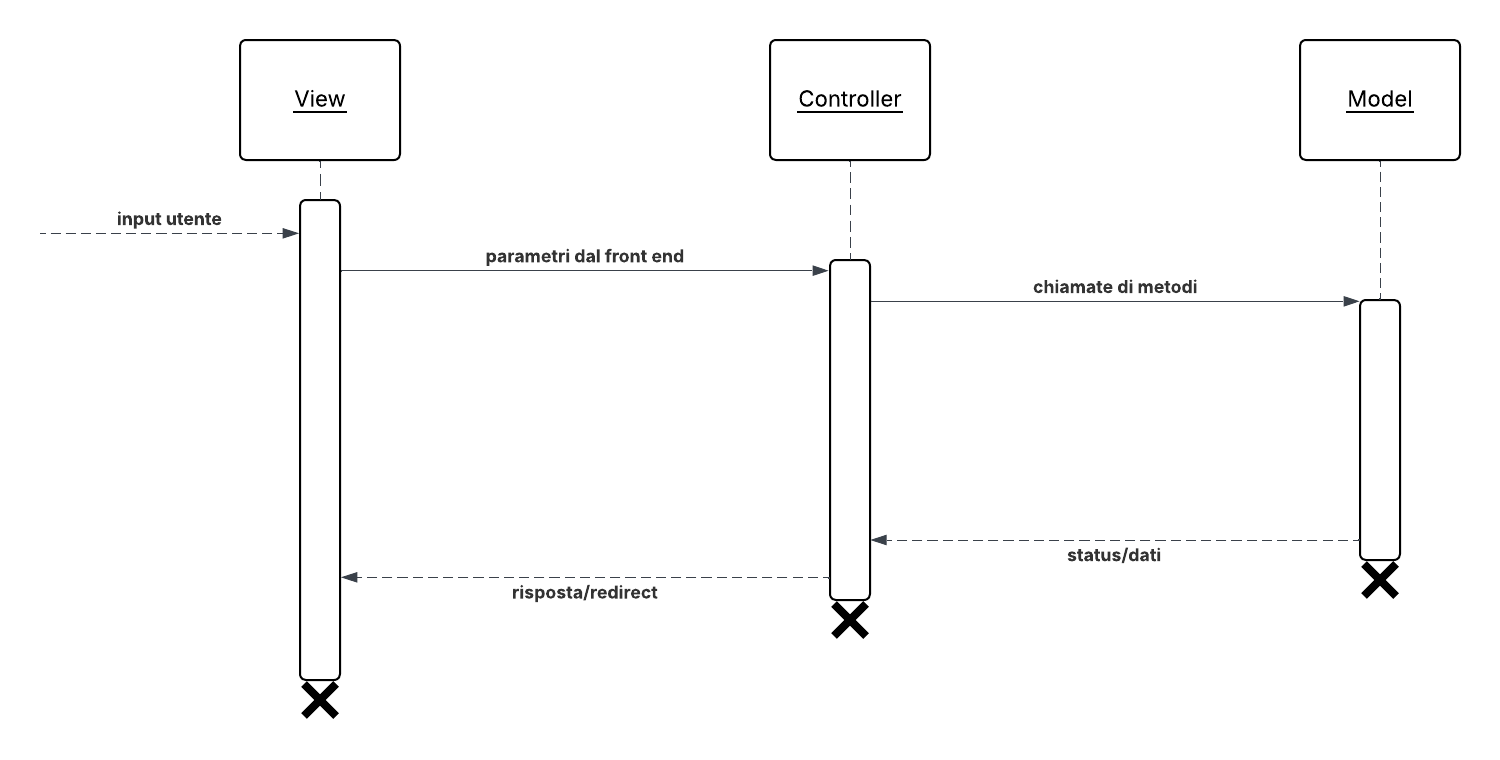
\includegraphics[width=0.8\linewidth]{Sequence Diagram pattern MVC.png}
\caption{Sequence diagram che illustra il flusso di interazione nel pattern MVC}
\label{fig:mvc-sequence}
\end{figure}
Infine nella root directory del progetto si trovano i file di supporto come il README.md inizializzato nel momento in cui è stata creata la repository gestita tramite
\textit{Gitflow}\cite{gitflow}, il CHANGELOG.md che serve a tenere presente le versioni dei rilasci 
e il Gemfile.rb che consiste nella lista delle gemme di Ruby aggiunte nel progetto ossia le librerie aggiuntive scaricate nel progetto.
Nel caso di questo software il client è stato sostituito con un client scritto in ReactJS e quindi di Ruby On Rails vengono usate principalmente le componenti
per costruire il server mentre le Views vengono utilizzate per definire template interni come le e-mails.
\subsection{Amazon Web Services}
Come anticipato prima, il blocco di servizi offerti da Amazon Web Services sono una componente molto importante dei software sviluppati in azienda.
AWS è una piattaforma di cloud computing che dispone di un catalogo di oltre 200 servizi IT on-demand accessibili via Internet con un modello di pagamento a consumo. Per questo software l'archiettura 
è stata realizzata attraverso \textit{Elastic Compute Cloud} (EC2) che permette di definire più istanze della stessa applicazione per far funzionare i tre ambienti del sito:
development ossia l'ambiente di sviluppo, staging che è l'ambiente in cui vengono rilasciati gli incrementi del software in modo che il cliente li possa testare
e production che è l'ambiente su cui funziona il sito ufficiale e che viene utilizzato dai clienti. L'accesso ai diversi server è gestito tramite \textit{Secure Shell Protocol}\cite{rfc4251} (SSH)
A livello di repository ogni istanza utilizza il codice dei branch omonimi e questo viene gestito attraverso \textit{CodePipeline}, un altro servizio di AWS che gestisce le fasi
di rilascio con uno script in Python e il servizio di containering di \textit{Docker}\cite{docker}. Questi containers sono monitorati dal servizio di \textit{Cloudwatch} che %TODO: citare e cercare Grafana
registra i log di ogni container, utili per le sessioni di debugging. Anche i database sono separati e istanziati attraverso il servizio \textit{Aurora and RDS} in modo che ogni
ambiente abbia il suo storage. Allo stesso modo di EC2, RDS permette di creare delle istanze alle quali si può accedere singolarmente tramite SSH per ogni database \textit{MYSQL}\cite{mysql}.
\textit{S3} è un servizio di storage in cloud che dà la possibilità di salvare media di qualsiasi tipo utilizzati nel software. Risulta particolarmente utile perchè permette di separare
la componente miscellanea dal software riducendone la dimensione effettiva. Si utilizza creando dei bucket che non sono niente meno di directory a cui ci si può collegare
da remoto e caricare, cancellare, aggiornare i media necessari. Infine viene utilizzato il servizio \textit{DynamoDB} che offre un database NoSQL serverless,
utile per immagazzinare dati non strutturati, nel caso di questo software si parla delle notifiche utilizzate per gestire il sistema di notifiche che segnalano lo stato di
avanzamento e conclusione dei processi asincroni ampliamente utilizzati nello sviluppo di questo modulo.
\subsection{Sidekiq}
I processi asincroni che d'ora in avanti saranno chiamati "job" sono gestiti attraverso una gemma di Ruby On Rails che si appoggia a \textit{Redis}\cite{redis_home} (REmote DIctionary Server), un
data store open source che può essere utilizzato come database, cache o broker di messaggi. Funziona salvando i dati nella RAM in forma di chiave-valore minimizzando le latenze nell'ordine dei microsecondi
dato che l'accesso ai dati salvati su disco è più lento rispetto all'accesso dei dati presenti in RAM. In questo caso Redis viene utilizzato per salvare le informazioni necessarie ai
job per svolgere le loro computazioni, di conseguenza ottimizza la velocità di esecuzione del job dato che l'accesso ai dati è molto veloce.
I vengono creati attraverso la gemma di Ruby On Rails di \textit{Sidekiq}\cite{sidekiq} che mette a disposizione un efficiente sistema di gestione di processi asincroni attraverso
metodi di una superclasse da sfruttare attraverso l'ereditarietà delle classi che implementano questo tipo di asincronismo. Il job viene astratto come un oggetto, dopotutto in
Ruby qualsiasi entità è un oggetto, con i suoi attributi fra cui i più rilevanti sono lo status, la data di creazione, di inzio e di fine processo e l'identificativo dell'oggetto che
implementa asincronismo. Il ciclo di vita è molto semplice: alla creazione ha status "running" e alla risoluzione diventa "complete" mentre se occorrono eccezioni durante la sua esecuzione
si imposta automaticamente uno status "error" e salva il messaggio d'errore in un campo apposito. La classe che implementa questo meccanismo deve possedere obbligatoriamente un metodo
"resolve\_job" che si potrà chiamare da qualsiasi punto del codice su un'istanza dell'oggetto e che svolgerà il suo task per poi concludere ed impostare lo stato "complete" aggiornando
anche il timestamp di fine. Spesso il front end avrà bisogno di ricevere un segnale che un certo processo ha concluso il suo task e l'esito finale di esso.
A questo scopo si usa un sistema di notifiche in tempo reale che comunichi lo stato finale del job ed eventualmente apportando dei dati che al front end in modo che quest'ultimo sappia
se poter proseguire con un redirect ad un'altra pagina mostrare un messaggio d'errore. Queste notifiche vengono salvate sul database di DynamoDB, servizio di AWS citato
prima e vengono cancellate dopo un dato periodo di tempo che sono state utilizzate. Questo sistema di asincronismo contribuisce al parallelismo di task uguali tra loro rendendo
l'applicazione più responsiva e migliorando le prestazioni.
% Citare OpenStruct molto importante
\section{Servizi esterni}
\subsection{Stripe}
Per la gestione del processo di pagamento, con particolare attenzione alle modalità di addebito ricorrente caratteristiche di un sistema di abbonamenti,
è stato integrato il servizio di \textit{Stripe}\cite{stripe} attraverso la gemma ufficiale per Ruby\cite{stripe_ruby_gem}. Il servizio offre un sistema di gestione dei pagamenti
basato su oggetti ed utilizzabile attraverso diversi linguaggi di programmazione oltre a Ruby fra cui Python, Java, .NET e altri. Si integra
bene con Ruby per il fatto che anche l'API di Stripe opera via oggetti identificati univocamente da object id e ha classi di oggetti con i loro attributi e metodi quindi allineandosi
perfettamente con il paradigma object oriented.
Offre molte classi per implementare flussi di pagamento e le più rilevanti nello sviluppo di questo modulo sono per esempio le classi Payment Intents, Subscriptions, Payment Methods,
Invoices, Tax Rate, Customers e tante altre che verranno illustrate approfonditamente assieme al flusso della funzionalità nel prossimo capitolo.
Stripe si è rilvelata una scelta vantaggiosa anche per il fatto che la gestione dei dati sensibili non è delegata al back end dell'applicazione ed è interamente
a carico del servizio stesso. Un altro punto di forza di questa API è la documentazione chiara\cite{stripe_api_reference} e la disponibilità di assistenza 24 ore su 24 da parte
del team di supporto di cui il team si è potuto avvalere per far fronte alle difficoltà incontrate durante il lavoro ad alcuni task.
\subsection{RabbitMQ}
L'analisi dei domini è stata affidata al servizio di \textit{RabbitMQ}\cite{rabbitmq}, un middleware message-oriented che implementa il protocollo \textit{Advanced Message Queuing Protocol}
(AMPQ) per gestire le richieste in entrata dall'applicazione e restituire in risposta gli stessi dati rielaborati.
L'integrazione avviene attraverso un server lato servizio che riceve le richieste inviate in formato JSON attraverso un canale che collega tale server e l'applicazione.
La comunicazione viene aperta dopo l'autenticazione avvenuta con successo tramite nome utente e password.
Il servizio opera principalmente secondo il pattern publish/subscribe. In pratica l'applicazione pubblica su una coda i dati interessati che devono essere elaborati,
poi questo dato pubblicato viene prelevato ed elaborato, tecnicamente consumato, dal server lato servizio che a fine elaborazione viene ripubblicato su una coda diversa
a cui l'applicazione si sottoscrive periodicamente per ricevere la risposta con i dati rielaborati.
\subsection{Axlsx}
\begin{figure}[h]
\centering
\includegraphics[width=1\linewidth]{Deployment Diagram.png}
\caption{Deployment diagram che mostra le interazioni fra i servizi utilizzati}
\label{fig:dep_diagram}
\end{figure}

\chapter{Funzionalità Sviluppata}

% Sistema o funzionalità sviluppata: casi d'uso, deployment diagram, comportamentale tipo activity
Il software essendo un e-commerce ha un flusso di utilizzo da parte di un utente generico molto semplice: cercare il prodotto desiderato,
aggiungerlo al carrello in caso lo si voglia acquistare, effettuare il pagamento e il check-out ed infine usufruire del prodotto acquistato.


\chapter{Valutazione}

Valutazione con testing in RSpec (https://github.com/simplecov-ruby/simplecov), questionario sul software per valutare
la bontà del prodotto e la soddisfazione degli utenti (va bene anche il team sviluppatori) -> da fare ad es su google forms o
microsoft forms con likert e domanda aperta per raccogliere feedback

\chapter{Conclusioni e Sviluppi Futuri}

conclusioni e sviluppi futuri


%% Fine dei capitoli normali, inizio dei capitoli-appendice (opzionali)
\appendix

%\part{Appendici}

% \chapter{Titolo della prima appendice}
% Sed purus libero, vestibulum ut nibh vitae, mollis ultricies augue. Pellentesque velit libero, tempor sed pulvinar non, fermentum eu leo. Duis posuere eleifend nulla eget sagittis. Nam laoreet accumsan rutrum. Interdum et malesuada fames ac ante ipsum primis in faucibus. Curabitur eget libero quis leo porttitor vehicula eget nec odio. Proin euismod interdum ligula non ultricies. Maecenas sit amet accumsan sapien.

%% Parte conclusiva del documento; tipicamente per riassunto, bibliografia e/o indice analitico.
\backmatter

%% Riassunto (opzionale)
%\summary
%Maecenas tempor elit sed arcu commodo, dapibus sagittis leo egestas. Praesent at ultrices urna. Integer et nibh in augue mollis facilisis sit amet eget magna. Fusce at porttitor sapien. Phasellus imperdiet, felis et molestie vulputate, mauris sapien tincidunt justo, in lacinia velit nisi nec ipsum. Duis elementum pharetra lorem, ut pellentesque nulla congue et. Sed eu venenatis tellus, pharetra cursus felis. Sed et luctus nunc. Aenean commodo, neque a aliquam bibendum, mauris augue fringilla justo, et scelerisque odio mi sit amet diam. Nulla at placerat nibh, nec rutrum urna. Donec ut egestas magna. Aliquam erat volutpat. Phasellus vestibulum justo sed purus mattis, vitae lacinia magna viverra. Nulla rutrum diam dui, vel semper mi mattis ac. Vestibulum ante ipsum primis in faucibus orci luctus et ultrices posuere cubilia Curae; Donec id vestibulum lectus, eget tristique est.

%% Bibliografia (praticamente obbligatoria)
\bibliographystyle{plain_\languagename}%% Carica l'omonimo file .bst, dove \languagename � la lingua attiva.
%% Nel caso in cui si usi un file .bib (consigliato)
\bibliography{thud}
%% Nel caso di bibliografia manuale, usare l'environment thebibliography.

%% Per l'indice analitico, usare il pacchetto makeidx (o analogo).

\end{document}
